% =============================================================================
% CAPÍTULO 2 - BLOQUE 2.4: ECOSISTEMA DE MODELOS ALTERNATIVOS:
% PESOS ABIERTOS (QWEN3-VL), ADAPTACIÓN DE VLMS Y ENTORNOS DE RECURSOS LIMITADOS
% =============================================================================

\subsection{Ecosistema de Modelos Alternativos: Pesos Abiertos (\textit{Open-Weights}) y Ejecución Local}
\label{subsec:modelos_locales}

\subsubsection{Las Dos Macrotendencias de 2026: APIs Propietarias Hiper-escaladas frente a Pesos Abiertos}
\label{subsubsec:macrotendencias_2026}

En el diseño de una plataforma de recuperación profunda de vídeo, la elección de la arquitectura del modelo de \textit{embedding} subyacente constituye el factor crítico que define los límites de escalabilidad, la precisión en la localización de eventos y el coste computacional del sistema \cite{gemini_emb2_docs}. %[cite: 4, 5]
El estado del arte tecnológico en 2026 se estructura en torno a dos macrotendencias complementarias \cite{qwen3_vl_emb2026, gemini_emb2_docs}: %
\begin{enumerate}
    \item \textbf{Modelos Propietarios Hiper-escalados vía API (\textit{Cloud}):} Representados por servicios como \textit{Google Gemini Embedding 2} (\texttt{gemini-embedding-2-preview}), donde la complejidad de la infraestructura de aceleradores (TPUs/GPUs) queda abstraída tras llamadas HTTP, ofreciendo espacios vectoriales masivos de hasta $3.072$ dimensiones con soporte nativo para vídeo, audio, imagen, texto y documentos PDF \cite{gemini_emb2_docs, openrouter_gemini_emb2}. %[cite: 3, 4]
    \item \textbf{Ecosistemas de Pesos Abiertos (\textit{Open-Weights}) y Despliegue Local:} Integrados por familias de modelos cuyos pesos neuronales son públicamente accesibles en repositorios como Hugging Face (destacando la serie \textbf{Qwen3-VL-Embedding} y \textbf{Qwen3-VL-Reranker}, arquitecturas como \textbf{ColQwen} y variantes ligeras de la familia \textbf{Gemma}), los cuales pueden ejecutarse en servidores locales propios o en instancias privadas sin depender de proveedores externos \cite{qwen3_vl_emb2026, hf_train_multimodal2026, prajwal2025multimodal}. %[cite: 3, 4]
\end{enumerate}

Un hallazgo fundamental documentado en la literatura del primer trimestre de 2026 es que las implementaciones de código abierto han logrado cerrar la brecha histórica de rendimiento frente a las APIs propietarias en tareas de recuperación multimodal \cite{qwen3_vl_emb2026, alphaxiv_qwen3}. %[cite: 4]
Esta convergencia técnica tiene una repercusión directa en el ámbito universitario e industrial: posibilita el diseño de infraestructuras de investigación académica y de producción que no dependen del pago continuo por inferencia (\textit{pay-per-token}) ni se ven estranguladas por límites diarios de peticiones, garantizando además la soberanía y privacidad absoluta sobre archivos de vídeo sensibles \cite{qwen3_vl_emb2026}. %[cite: 3, 4]

La Figura~\ref{fig:ecosistema_cloud_vs_open} presenta la taxonomía comparada de ambas corrientes tecnológicas dentro del panorama de modelos fundacionales multimodales de 2026. %[cite: 3, 4]

\begin{figure}[htbp]
\centering
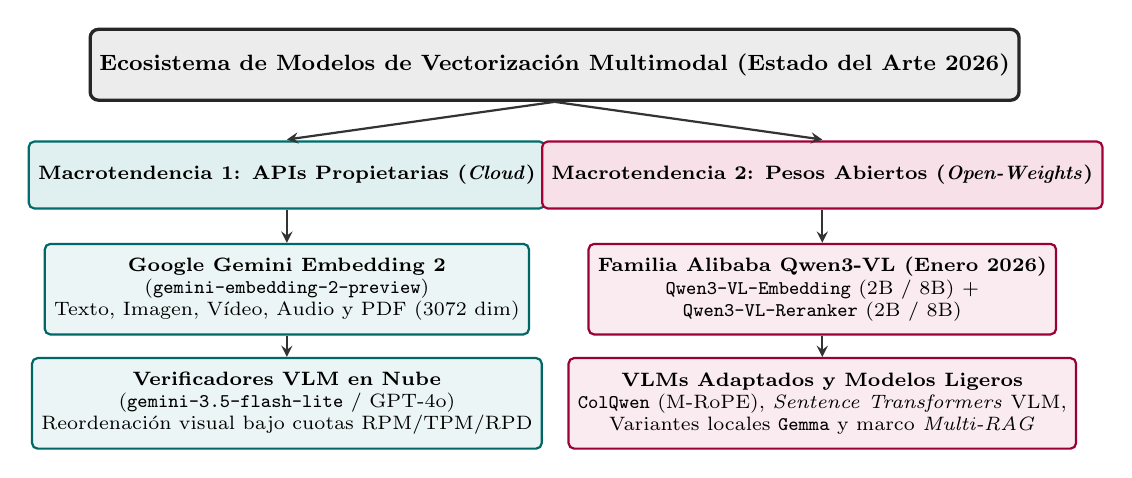
\begin{tikzpicture}[
    node distance=0.5cm and 0.6cm,
    rootbox/.style={rectangle, draw=black!85, fill=gray!15, very thick, minimum width=7.8cm, minimum height=0.9cm, align=center, font=\footnotesize\bfseries, rounded corners=3pt},
    branchbox/.style={rectangle, draw=blue!80!black, fill=blue!10, thick, minimum width=6.0cm, minimum height=0.85cm, align=center, font=\scriptsize\bfseries, rounded corners=2pt},
    leafcloud/.style={rectangle, draw=teal!80!black, fill=teal!8, thick, minimum width=5.8cm, minimum height=1.15cm, align=center, font=\scriptsize, rounded corners=2pt},
    leafopen/.style={rectangle, draw=purple!80!black, fill=purple!8, thick, minimum width=5.8cm, minimum height=1.15cm, align=center, font=\scriptsize, rounded corners=2pt},
    arrow/.style={-stealth, thick, draw=black!80}
]
\node[rootbox] (root) at (0, 3.2) {Ecosistema de Modelos de Vectorización Multimodal (Estado del Arte 2026)};

% Ramas principales
\node[branchbox, draw=teal!85!black, fill=teal!12] (cloud) at (-3.4, 1.8) {Macrotendencia 1: APIs Propietarias (\textit{Cloud})};
\node[branchbox, draw=purple!85!black, fill=purple!12] (open) at (3.4, 1.8) {Macrotendencia 2: Pesos Abiertos (\textit{Open-Weights})};

\draw[arrow] (root.south) -- (-3.4, 2.25);
\draw[arrow] (root.south) -- (3.4, 2.25);

% Hojas Cloud
\node[leafcloud] (c1) at (-3.4, 0.35) {\textbf{Google Gemini Embedding 2}\\(\texttt{gemini-embedding-2-preview})\\Texto, Imagen, Vídeo, Audio y PDF (3072 dim)};
\node[leafcloud] (c2) at (-3.4, -1.1) {\textbf{Verificadores VLM en Nube}\\(\texttt{gemini-3.5-flash-lite} / GPT-4o)\\Reordenación visual bajo cuotas RPM/TPM/RPD};

\draw[arrow] (cloud) -- (c1);
\draw[arrow] (c1) -- (c2);

% Hojas Open-Weights
\node[leafopen] (o1) at (3.4, 0.35) {\textbf{Familia Alibaba Qwen3-VL (Enero 2026)}\\ \texttt{Qwen3-VL-Embedding} (2B / 8B) +\\ \texttt{Qwen3-VL-Reranker} (2B / 8B)};
\node[leafopen] (o2) at (3.4, -1.1) {\textbf{VLMs Adaptados y Modelos Ligeros}\\ \texttt{ColQwen} (M-RoPE), \textit{Sentence Transformers} VLM,\\Variantes locales \texttt{Gemma} y marco \textit{Multi-RAG}};

\draw[arrow] (open) -- (o1);
\draw[arrow] (o1) -- (o2);
\end{tikzpicture}
\caption{Clasificación de las arquitecturas de modelos fundacionales para Video RAG en 2026: coexistencia de modelos hiper-escalados servidos mediante API comercial frente a ecosistemas de pesos abiertos desplegables en infraestructura local \cite{gemini_emb2_docs, qwen3_vl_emb2026, multi_rag2025}.} %[cite: 3, 4]
\label{fig:ecosistema_cloud_vs_open}
\end{figure}

\subsubsection{La Familia Qwen3-VL: Recuperación y Reordenación Multimodal a Escala Masiva}
\label{subsubsec:familia_qwen3_vl}

En el espectro del software libre y los modelos de pesos abiertos, la referencia técnica para la recuperación de información multimodal viene marcada por el lanzamiento en enero de 2026 de la serie \textbf{Qwen3-VL-Embedding} y \textbf{Qwen3-VL-Reranker} por parte del grupo de investigación de Alibaba \cite{qwen3_vl_emb2026, qwen3_vl_blog2026, qwen3_vl_github2026}. %[cite: 4]
Publicados oficialmente en configuraciones de $2.000$ millones (\texttt{Qwen/Qwen3-VL-Embedding-2B}) y $8.000$ millones de parámetros (\texttt{Qwen/Qwen3-VL-Embedding-8B}), junto con adaptaciones especializadas en recuperación de documentos visuales (\texttt{tomaarsen/Qwen3-VL-Embedding-2B-vdr}), estos modelos abordan el problema del RAG sobre grandes repositorios de vídeo mediante un diseño acoplado en dos etapas que supera las limitaciones de latencia de los sistemas generativos directos \cite{qwen3_vl_emb2026, hf_qwen3_2b, hf_qwen3_8b, hf_qwen3_vdr}. %[cite: 4]

\paragraph{Primera Etapa (\texttt{Qwen3-VL-Embedding}):}
Actúa como un codificador denso de doble torre (\textit{Bi-Encoder}) construido sobre la arquitectura base de visión y lenguaje de la familia Qwen3 \cite{qwen3_vl_emb2026, learnopencv_qwen3}. %[cite: 4]
Gracias a la integración nativa de \textit{Multimodal Rotary Position Embeddings} (M-RoPE), el modelo proyecta parches y teselas visuales de imágenes y secuencias de vídeo directamente hacia el mismo espacio semántico continuo del lenguaje sin requerir preprocesamiento OCR intermedio \cite{prajwal2025multimodal, qwen3_vl_emb2026}. %[cite: 4]
Estos vectores se almacenan en bases de datos vectoriales como Qdrant o Milvus, permitiendo realizar búsquedas semánticas directas sobre vídeo bruto a gran velocidad \cite{qwen3_vl_emb2026}. %[cite: 3, 4]

\paragraph{Segunda Etapa (\texttt{Qwen3-VL-Reranker}) y Resolución de Consultas Composicionales:}
El aporte arquitectónico más relevante de la investigación del equipo Qwen radica en demostrar empíricamente por qué un \textit{Bi-Encoder} aislado resulta insuficiente ante consultas visualmente complejas \cite{learnopencv_qwen3, qwen3_vl_emb2026}. %[cite: 4]
Los codificadores de doble torre tienden a degradar su precisión ante \textbf{consultas altamente composicionales}, perdiendo relaciones espaciales, direccionales o de atributos cruzados; un caso paradigmático documentado en la literatura es la búsqueda de un evento descrito como \textit{``una persona vistiendo una chaqueta roja que se aleja de una furgoneta blanca''} \cite{learnopencv_qwen3}. %[cite: 4]
En un \textit{Bi-Encoder}, un fragmento de vídeo donde aparezca una furgoneta roja y una persona con chaqueta blanca acercándose a ella puede arrojar una similitud del coseno artificialmente alta debido a la presencia conjunta de los mismos sustantivos y colores en el vector global. %[cite: 4]

Para erradicar estos falsos positivos composicionales, \texttt{Qwen3-VL-Reranker} actúa como un filtro de alta precisión sobre el subconjunto top-$K$ recuperado en la primera fase \cite{learnopencv_qwen3, qwen3_vl_emb2026}. %[cite: 4]
Operando bajo una arquitectura de Torre Única (\textit{Cross-Encoder}), el modelo ingiere simultáneamente la consulta textual $Q$ y el fragmento multimedia candidato $D_k$, permitiendo que sus capas de atención cruzada (\textit{Cross-Attention}) interactúen de manera bidireccional y profunda entre cada \textit{token} léxico del texto y cada parche espacial de los fotogramas del vídeo \cite{learnopencv_qwen3, qwen3_vl_emb2026}. %[cite: 4]
En lugar de emitir un vector de representación, la red finaliza prediciendo según la Ecuación~\eqref{eq:qwen3_reranker_logit} un \textbf{\textit{logit} de probabilidad absoluta} que cuantifica la relevancia exacta de la coincidencia entre el evento visual y la estructura sintáctica de la consulta, maximizando la precisión en las primeras posiciones del ranking \cite{learnopencv_qwen3, qwen3_vl_emb2026}. %[cite: 4]

\begin{equation}
P(\text{Relevante} \mid Q, D_k) = \sigma\!\left(z_{\text{logit}}(Q, D_k)\right) = \frac{1}{1 + \exp\!\left(-\mathbf{w}^\top \mathbf{h}_{\text{Cross-Attention}}(Q, D_k)\right)}
\label{eq:qwen3_reranker_logit}
\end{equation} %[cite: 4]

La Figura~\ref{fig:qwen3_vl_composicional} ilustra el mecanismo mediante el cual \texttt{Qwen3-VL-Reranker} desambigua relaciones espaciales y de atributos sobre los candidatos recuperados por \texttt{Qwen3-VL-Embedding}. %[cite: 4]

\begin{figure}[htbp]
\centering
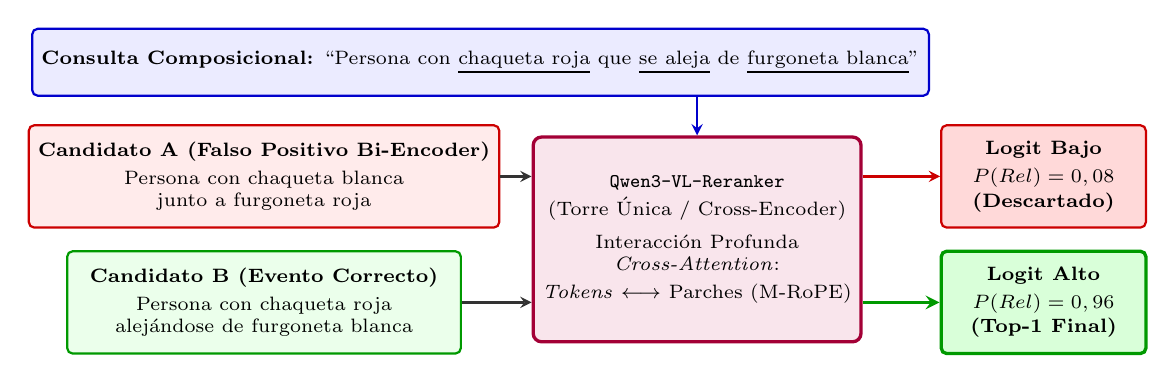
\begin{tikzpicture}[
    node distance=0.5cm and 0.65cm,
    qbox/.style={rectangle, draw=blue!80!black, fill=blue!8, thick, minimum width=10.6cm, minimum height=0.85cm, align=center, font=\scriptsize, rounded corners=2pt},
    candbad/.style={rectangle, draw=red!80!black, fill=red!8, thick, minimum width=5.0cm, minimum height=1.3cm, align=center, font=\scriptsize, rounded corners=2pt},
    candgood/.style={rectangle, draw=green!60!black, fill=green!8, thick, minimum width=5.0cm, minimum height=1.3cm, align=center, font=\scriptsize, rounded corners=2pt},
    attbox/.style={rectangle, draw=purple!85!black, fill=purple!10, very thick, minimum width=3.8cm, minimum height=2.6cm, align=center, font=\scriptsize, rounded corners=3pt},
    outbad/.style={rectangle, draw=red!80!black, fill=red!15, thick, minimum width=2.6cm, minimum height=1.3cm, align=center, font=\scriptsize\bfseries, rounded corners=2pt},
    outgood/.style={rectangle, draw=green!60!black, fill=green!15, very thick, minimum width=2.6cm, minimum height=1.3cm, align=center, font=\scriptsize\bfseries, rounded corners=2pt},
    arrow/.style={-stealth, thick, draw=black!80}
]
% Consulta composicional
\node[qbox] (query) at (-2.25, 2.15) {\textbf{Consulta Composicional:} ``Persona con \underline{chaqueta roja} que \underline{se aleja} de \underline{furgoneta blanca}''};

% Candidatos del Bi-Encoder (Top-K)
\node[candbad] (c1) at (-5.0, 0.70) {\textbf{Candidato A (Falso Positivo Bi-Encoder)}\\[2pt]Persona con chaqueta blanca\\junto a furgoneta roja};
\node[candgood] (c2) at (-5.0, -0.90) {\textbf{Candidato B (Evento Correcto)}\\[2pt]Persona con chaqueta roja\\alejándose de furgoneta blanca};

% Torre Única Qwen3-VL-Reranker
\node[attbox] (rerank) at (0.5, -0.10) {\textbf{\texttt{Qwen3-VL-Reranker}}\\[2pt]
(Torre Única / Cross-Encoder)\\[4pt]
Interacción Profunda\\
\textit{Cross-Attention}:\\[2pt]
\textit{Tokens} $\longleftrightarrow$ Parches (M-RoPE)};

% Salidas de Logit
\node[outbad] (s1) at (4.9, 0.70) {\textbf{Logit Bajo}\\[2pt]$P(\text{Rel}) = 0,08$\\[1pt](Descartado)};
\node[outgood] (s2) at (4.9, -0.90) {\textbf{Logit Alto}\\[2pt]$P(\text{Rel}) = 0,96$\\[1pt](\textbf{Top-1 Final})};

\draw[arrow, blue!80!black, thick] (query.south -| rerank.north) -- (rerank.north);
\draw[arrow] (c1.east) -- (rerank.west |- c1.east);
\draw[arrow] (c2.east) -- (rerank.west |- c2.east);
\draw[arrow, red!80!black, thick] (rerank.east |- s1.west) -- (s1.west);
\draw[arrow, green!60!black, very thick] (rerank.east |- s2.west) -- (s2.west);
\end{tikzpicture}
\caption{Resolución de consultas altamente composicionales mediante la arquitectura en dos etapas de la familia Qwen3-VL: mientras el \textit{Bi-Encoder} puede recuperar candidatos con atributos invertidos, las capas de \textit{Cross-Attention} de \texttt{Qwen3-VL-Reranker} vinculan cada adjetivo y acción con su parche visual exacto para predecir el \textit{logit} de probabilidad real \cite{learnopencv_qwen3, qwen3_vl_emb2026}.} %[cite: 4]
\label{fig:qwen3_vl_composicional}
\end{figure}

\subsubsection{Adaptación de Modelos Visuales (ColQwen y Sentence Transformers) y Entornos Restringidos (\textit{Multi-RAG})}
\label{subsubsec:adaptacion_vlms_multirag}

Más allá de la serie Qwen3-VL, la comunidad investigadora ha consolidado metodologías reproducibles para entrenar y ajustar (\textit{finetuning}) modelos de \textit{embeddings} y \textit{rerankers} multimodales a partir de arquitecturas de lenguaje visual preexistentes, tal y como documenta el marco de \textit{Sentence Transformers} multimodales de Hugging Face \cite{hf_train_multimodal2026, hf_qwen3_paper}. %[cite: 4]

Dentro de esta línea destaca \textbf{ColQwen}, una arquitectura que integra directamente \textit{Multimodal Rotary Position Embeddings} (M-RoPE) sobre el codificador visual para proyectar parches y teselas de documentos complejos, gráficos, ecografías o diapositivas con ecuaciones matemáticas hacia el espacio latente del lenguaje sin pasar por motores OCR \cite{prajwal2025multimodal}. %[cite: 4]
El impacto estructural de este diseño en entornos empresariales y académicos radica en la eliminación de las antiguas cadenas de dependencias compuestas por múltiples APIs de bajo nivel: el modelo fundacional interactúa directamente con la señal visual sin pulir y mapea inherentemente el significado cruzado sin intervención ortográfica, suprimiendo la cascada de errores que un OCR defectuoso propagaba hacia las etapas posteriores del razonamiento algorítmico \cite{prajwal2025multimodal}. %[cite: 4]

La Figura~\ref{fig:finetuning_vlm_to_embedding} esquematiza este flujo de adaptación de un VLM hacia un motor de indexación directa de parches visuales. %[cite: 4]

\begin{figure}[htbp]
\centering
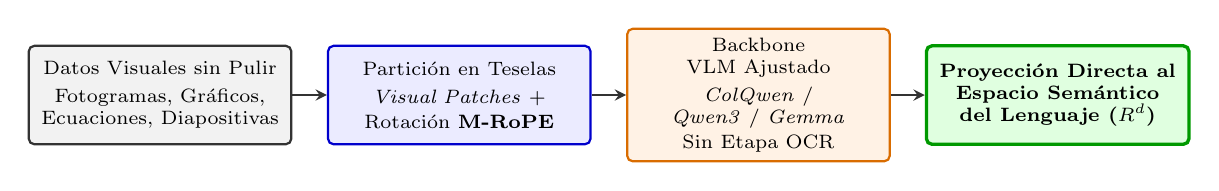
\begin{tikzpicture}[
    rawbox/.style={rectangle, draw=black!80, fill=gray!10, thick, text width=3.1cm, minimum height=1.25cm, align=center, font=\scriptsize, rounded corners=2pt},
    patchbox/.style={rectangle, draw=blue!80!black, fill=blue!8, thick, text width=3.1cm, minimum height=1.25cm, align=center, font=\scriptsize, rounded corners=2pt},
    trainbox/.style={rectangle, draw=orange!85!black, fill=orange!10, thick, text width=3.1cm, minimum height=1.25cm, align=center, font=\scriptsize, rounded corners=2pt},
    spacebox/.style={rectangle, draw=green!60!black, fill=green!12, very thick, text width=3.1cm, minimum height=1.25cm, align=center, font=\scriptsize\bfseries, rounded corners=2pt},
    arrow/.style={-stealth, thick, draw=black!80}
]
\node[rawbox] (in) at (-5.7, 0) {Datos Visuales sin Pulir\\[2pt]{\scriptsize Fotogramas, Gráficos,\\Ecuaciones, Diapositivas}};

\node[patchbox] (vit) at (-1.9, 0) {Partición en Teselas\\[2pt]{\scriptsize \textit{Visual Patches}} +\\[1pt]Rotación \textbf{M-RoPE}};

\node[trainbox] (ft) at (1.9, 0) {Backbone VLM Ajustado\\[2pt]{\scriptsize \textit{ColQwen} / \textit{Qwen3} / \textit{Gemma}}\\[1pt]Sin Etapa OCR};

\node[spacebox] (out) at (5.7, 0) {Proyección Directa al\\Espacio Semántico\\del Lenguaje ($\mathbb{R}^d$)};

\draw[arrow] (in) -- (vit);
\draw[arrow] (vit) -- (ft);
\draw[arrow] (ft) -- (out);
\end{tikzpicture}
\caption{Flujo de codificación visual directa en arquitecturas como \textit{ColQwen} y \textit{Sentence Transformers} multimodales: la combinación de teselas visuales con codificación posicional M-RoPE proyecta diapositivas, gráficos y escenas de vídeo directamente al espacio del lenguaje, eliminando el preprocesamiento intermedio mediante OCR \cite{prajwal2025multimodal, hf_train_multimodal2026}.} %[cite: 4]
\label{fig:finetuning_vlm_to_embedding}
\end{figure}

De manera complementaria, cuando los sistemas deben ejecutarse en dispositivos locales con recursos limitados (escenario donde se ubican las variantes ligeras de ejecución local como la familia \textbf{Gemma} y marcos de trabajo en tiempo real), la literatura reciente aporta la arquitectura \textbf{Multi-RAG} (\textit{A Multimodal Retrieval-Augmented Generation System for Adaptive Video Understanding}) \cite{multi_rag2025, arxiv_adaptive_2505}. %[cite: 3, 4]
\textit{Multi-RAG} introduce una capa de aplicación práctica orientada a la comprensión adaptativa de flujos de vídeo capturados en tiempo real, concebida específicamente como soporte cognitivo para la interacción humano-robot en contextos dinámicos y no estructurados del mundo real \cite{multi_rag2025, arxiv_adaptive_2505}. %[cite: 4]
La aportación fundamental de \textit{Multi-RAG} demuestra que los \textit{embeddings} multimodales son capaces de mantener una inferencia semántica de alto rendimiento incluso cuando la entrada visual se ve temporalmente degradada, ocluida o limitada, validando la robustez de estas representaciones vectoriales en escenarios con fuertes restricciones de recursos computacionales \cite{multi_rag2025, arxiv_adaptive_2505}. %[cite: 4]

\subsubsection{Evaluación en Bancos de Pruebas Masivos (MMEB-V2 y MVEB) y Compromisos de Despliegue}
\label{subsubsec:benchmarks_mmeb_mveb}

Para cuantificar de manera objetiva y estandarizada la capacidad de recuperación de estos modelos fundacionales sobre vídeo, audio y documentos complejos, la comunidad científica ha establecido entre 2025 y 2026 dos bancos de pruebas (\textit{benchmarks}) masivos de referencia \cite{qwen3_vl_emb2026, alphaxiv_qwen3}: %[cite: 3, 4]
\begin{itemize}
    \item \textbf{MMEB-V2 (\textit{Massive Multimodal Embedding Benchmark V2}, 2025):} Amplió la evaluación tradicional de representaciones estáticas texto-imagen para incorporar tareas exigentes de recuperación de fragmentos de vídeo y documentos estructurados (archivos PDF) \cite{qwen3_vl_emb2026, alphaxiv_qwen3}. %[cite: 3, 4]
    Desde el punto de vista metodológico, las métricas empleadas en \textit{MMEB-V2} para clasificación de imágenes y recuperación de vídeo se fundamentan predominantemente en \textbf{\textit{Recall@1}} y \textbf{\textit{Hit@1}}, mientras que los dominios de recuperación de documentos visuales evalúan el ordenamiento mediante \textbf{\textit{NDCG@5}} \cite{alphaxiv_qwen3, qwen3_vl_emb2026}. %[cite: 4]
    \item \textbf{MVEB (\textit{Massive Video Embedding Benchmark}, 2026):} Constituye el estándar específico de evaluación temporal más exhaustivo hasta la fecha, consolidando más de $180$ tareas diferenciadas diseñadas para poner a prueba cómo los modelos de \textit{embeddings} recuperan eventos combinando secuencias de vídeo y pistas de audio. %[cite: 3]
\end{itemize}

A partir de la evidencia empírica recogida en estos bancos de pruebas y de las especificaciones operativas de cada ecosistema, un ingeniero de datos debe ponderar los compromisos arquitectónicos (\textit{trade-offs}) entre desplegar la solución apoyándose en una API propietaria en la nube frente a alojar modelos de pesos abiertos en infraestructura local \cite{gemini_emb2_docs, qwen3_vl_emb2026}. %[cite: 3, 4]
La Figura~\ref{fig:tradeoff_cloud_local_tfm} sintetiza la matriz de decisión técnica entre ambos enfoques. %[cite: 3, 4]

\begin{figure}[htbp]
\centering
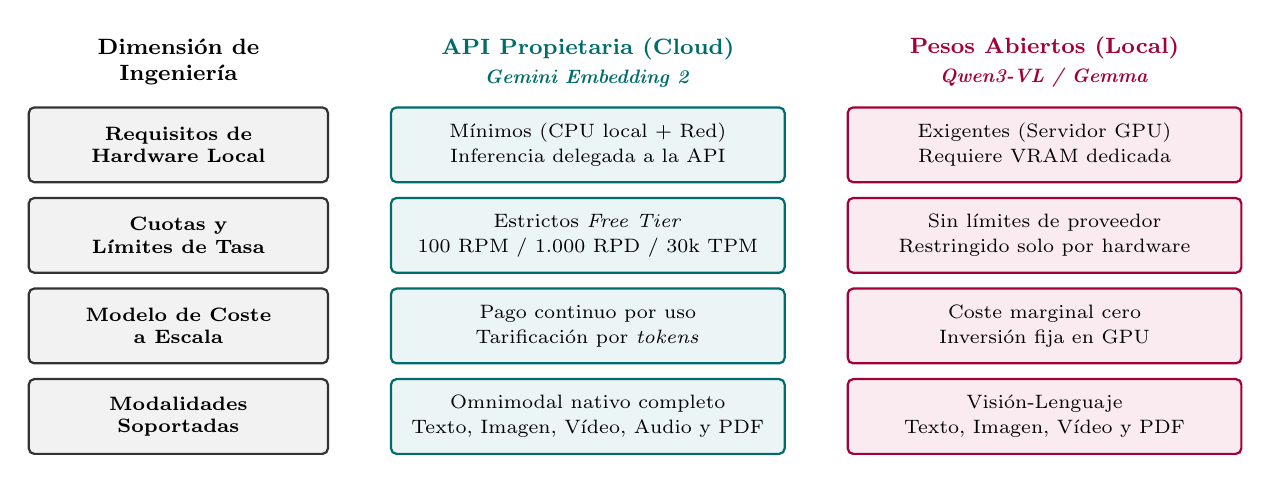
\begin{tikzpicture}[
    node distance=0.5cm and 0.8cm,
    axisbox/.style={rectangle, draw=black!80, fill=gray!10, thick, minimum width=3.8cm, minimum height=0.95cm, align=center, font=\scriptsize\bfseries, rounded corners=2pt},
    cloudnode/.style={rectangle, draw=teal!85!black, fill=teal!8, thick, minimum width=5.0cm, minimum height=0.95cm, align=center, font=\scriptsize, rounded corners=2pt},
    localnode/.style={rectangle, draw=purple!85!black, fill=purple!8, thick, minimum width=5.0cm, minimum height=0.95cm, align=center, font=\scriptsize, rounded corners=2pt}
]
% Encabezados
\node[font=\footnotesize\bfseries, align=center] at (-5.8, 2.35) {Dimensión de\\Ingeniería};
\node[font=\footnotesize\bfseries, teal!85!black, align=center] at (-0.6, 2.35) {API Propietaria (Cloud)\\[1pt]{\scriptsize \textit{Gemini Embedding 2}}};
\node[font=\footnotesize\bfseries, purple!85!black, align=center] at (5.2, 2.35) {Pesos Abiertos (Local)\\[1pt]{\scriptsize \textit{Qwen3-VL / Gemma}}};

% Fila 1: Hardware local
\node[axisbox] (a1) at (-5.8, 1.30) {Requisitos de\\Hardware Local};
\node[cloudnode] (c1) at (-0.6, 1.30) {Mínimos (CPU local + Red)\\[1pt]Inferencia delegada a la API};
\node[localnode] (l1) at (5.2, 1.30) {Exigentes (Servidor GPU)\\[1pt]Requiere VRAM dedicada};

% Fila 2: Límites de Tasa
\node[axisbox] (a2) at (-5.8, 0.15) {Cuotas y\\Límites de Tasa};
\node[cloudnode] (c2) at (-0.6, 0.15) {Estrictos \textit{Free Tier}\\[1pt]100 RPM / 1.000 RPD / 30k TPM};
\node[localnode] (l2) at (5.2, 0.15) {Sin límites de proveedor\\[1pt]Restringido solo por hardware};

% Fila 3: Coste Operativo
\node[axisbox] (a3) at (-5.8, -1.00) {Modelo de Coste\\a Escala};
\node[cloudnode] (c3) at (-0.6, -1.00) {Pago continuo por uso\\[1pt]Tarificación por \textit{tokens}};
\node[localnode] (l3) at (5.2, -1.00) {Coste marginal cero\\[1pt]Inversión fija en GPU};

% Fila 4: Cobertura Modal
\node[axisbox] (a4) at (-5.8, -2.15) {Modalidades\\Soportadas};
\node[cloudnode] (c4) at (-0.6, -2.15) {Omnimodal nativo completo\\[1pt]Texto, Imagen, Vídeo, Audio y PDF};
\node[localnode] (l4) at (5.2, -2.15) {Visión-Lenguaje\\[1pt]Texto, Imagen, Vídeo y PDF};
\end{tikzpicture}
\caption{Comparativa de compromisos de ingeniería entre el despliegue sobre API propietaria en la nube y la ejecución local con modelos de pesos abiertos para sistemas de recuperación de vídeo \cite{gemini_emb2_docs, qwen3_vl_emb2026}.} %[cite: 3, 4]
\label{fig:tradeoff_cloud_local_tfm}
\end{figure}

El Cuadro~\ref{tab:ecosistema_modelos_2026} consolida las especificaciones técnicas de las familias de modelos analizadas en este bloque, detallando su topología, capacidades modales y métricas de referencia en el estado del arte. %[cite: 3, 4]

\begin{table}[htbp]
\centering
\small
\setlength{\tabcolsep}{4.5pt}
\caption{Síntesis comparativa de las principales arquitecturas y modelos del ecosistema multimodal analizados en la literatura (2025-2026) \cite{gemini_emb2_docs, qwen3_vl_emb2026, multi_rag2025, prajwal2025multimodal}.} %[cite: 3, 4]
\label{tab:ecosistema_modelos_2026}
\begin{tabularx}{\linewidth}{>{\raggedright\arraybackslash}p{3.2cm} >{\raggedright\arraybackslash}p{2.2cm} >{\raggedright\arraybackslash}p{2.4cm} >{\raggedright\arraybackslash}X >{\raggedright\arraybackslash}X}
\toprule
\textbf{Modelo / Sistema} & \textbf{Despliegue} & \textbf{Topología} & \textbf{Innovación Clave} & \textbf{Evaluación / Rol Principal} \\
\midrule
Gemini Embedding 2 & Cloud (API) & Bi-Encoder & Omnimodal nativo (3.072 dim) & \textit{Baseline} PoC sin GPU local \\
Qwen3-VL-Embedding & Local (2B/8B) & Bi-Encoder & M-RoPE + Vectores MRL & Recuperación masiva en MMEB-V2 \\
Qwen3-VL-Reranker & Local (2B/8B) & Cross-Encoder & \textit{Cross-Attention} + Logit & Consultas composicionales (Top-$K$) \\
ColQwen & Local (Open) & Interacción ViT & Parches directos con M-RoPE & Eliminación total de etapa OCR \\
Multi-RAG / Gemma & Local / Edge & Adaptativo & Inferencia ante vídeo degradado & Robótica y recursos restringidos \\
\bottomrule
\end{tabularx}
\end{table}

Como demuestra este análisis comparado, mientras que los modelos de pesos abiertos como \textit{Qwen3-VL-Embedding} y \textit{Qwen3-VL-Reranker} constituyen la opción óptima cuando se dispone de servidores con aceleración GPU dedicada y se requiere indexar volúmenes masivos sin coste por inferencia, el uso de \textit{Gemini Embedding 2} junto con una base de datos vectorial embebida como Qdrant permite desarrollar y validar una Prueba de Concepto omnimodal completa en ordenadores convencionales sin hardware gráfico especializado, siempre que se instrumenten los controles de concurrencia y cuota detallados en la sección anterior \cite{gemini_emb2_docs, qwen3_vl_emb2026}. %[cite: 3, 4]